\begin{figure}[t!]
    \centering
    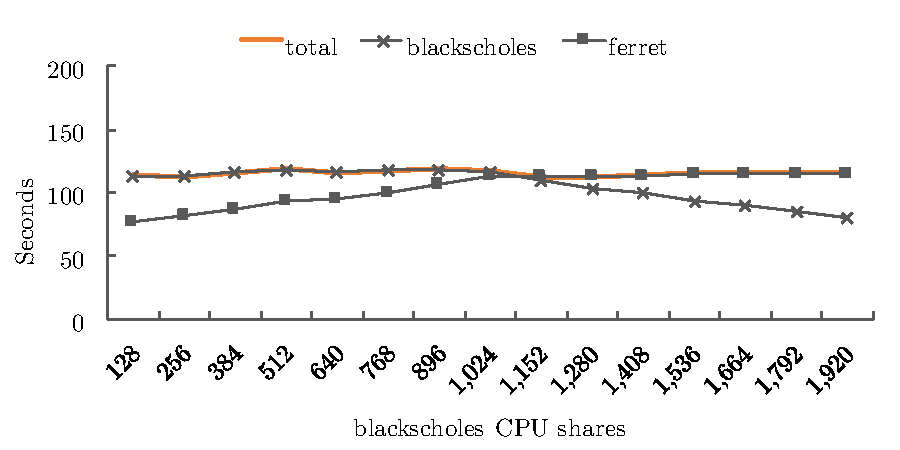
\includegraphics[width=8cm,height=4cm]{fig/without-application.pdf}
    \caption{Improving overall performance is difficult without true cooperation from applications.  In this simple example, we have a total of 2048 shares of CPU time that we divide among two applications, \texttt{blackscholes} and \texttt{ferret}, that start at the same time. We use Linux control groups to enforce that the two applications will have roughly the same ratio of time on CPU as the ratio of their weights. We can manipulate an application's resources with CPU shares, but we cannot alter application behavior via this mechanism and as a result, minimally impact the total execution time (orange, for those with color).}
    \label{fig:naive-cooperation}
\end{figure}